\documentclass{standalone}
\usepackage{tikz}
\usepackage{ctex,siunitx}
\setCJKmainfont{Noto Serif CJK SC}
\usepackage{tkz-euclide}
\usepackage{amsmath}
\usetikzlibrary{patterns, calc}
\usetikzlibrary {decorations.pathmorphing, decorations.pathreplacing, decorations.shapes,}

\begin{document}
\small
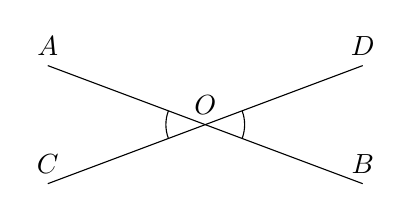
\begin{tikzpicture}[>=stealth,scale=1]
  \tkzSetUpPoint[fill=black]
  % \useasboundingbox(-1,-0.75)rectangle(3.7,1.4);
	\tkzDefPoints{-2/.75/A, 2/-.75/B, -2/-.75/C, 2/.75/D,0/0/O}
	\tkzLabelPoints[above](A,B,C,D,O)
	\draw(A)--(B);
	\draw(C)--(D);
	\tkzMarkAngles[mark=none, size=.5](A,O,C B,O,D)
\end{tikzpicture}
\end{document}